\subsection{Comparison with Malware Dataset}
\label{sec:analysisLLLComparisonMalware}

We analyzed when this metric is effective for detecting these four attacks 
(described in \cref{ch:AnalysisRecentAttacks}) and when it is not indicative.
To do so, we used a specific figure for each attack, as explained in \cref{sec:Figure2}.

\subsection*{Attack A: Malicious Windows DLL}
\label{sec:analysisLLLAttackA}

\begin{figure}[H]
    \centering
    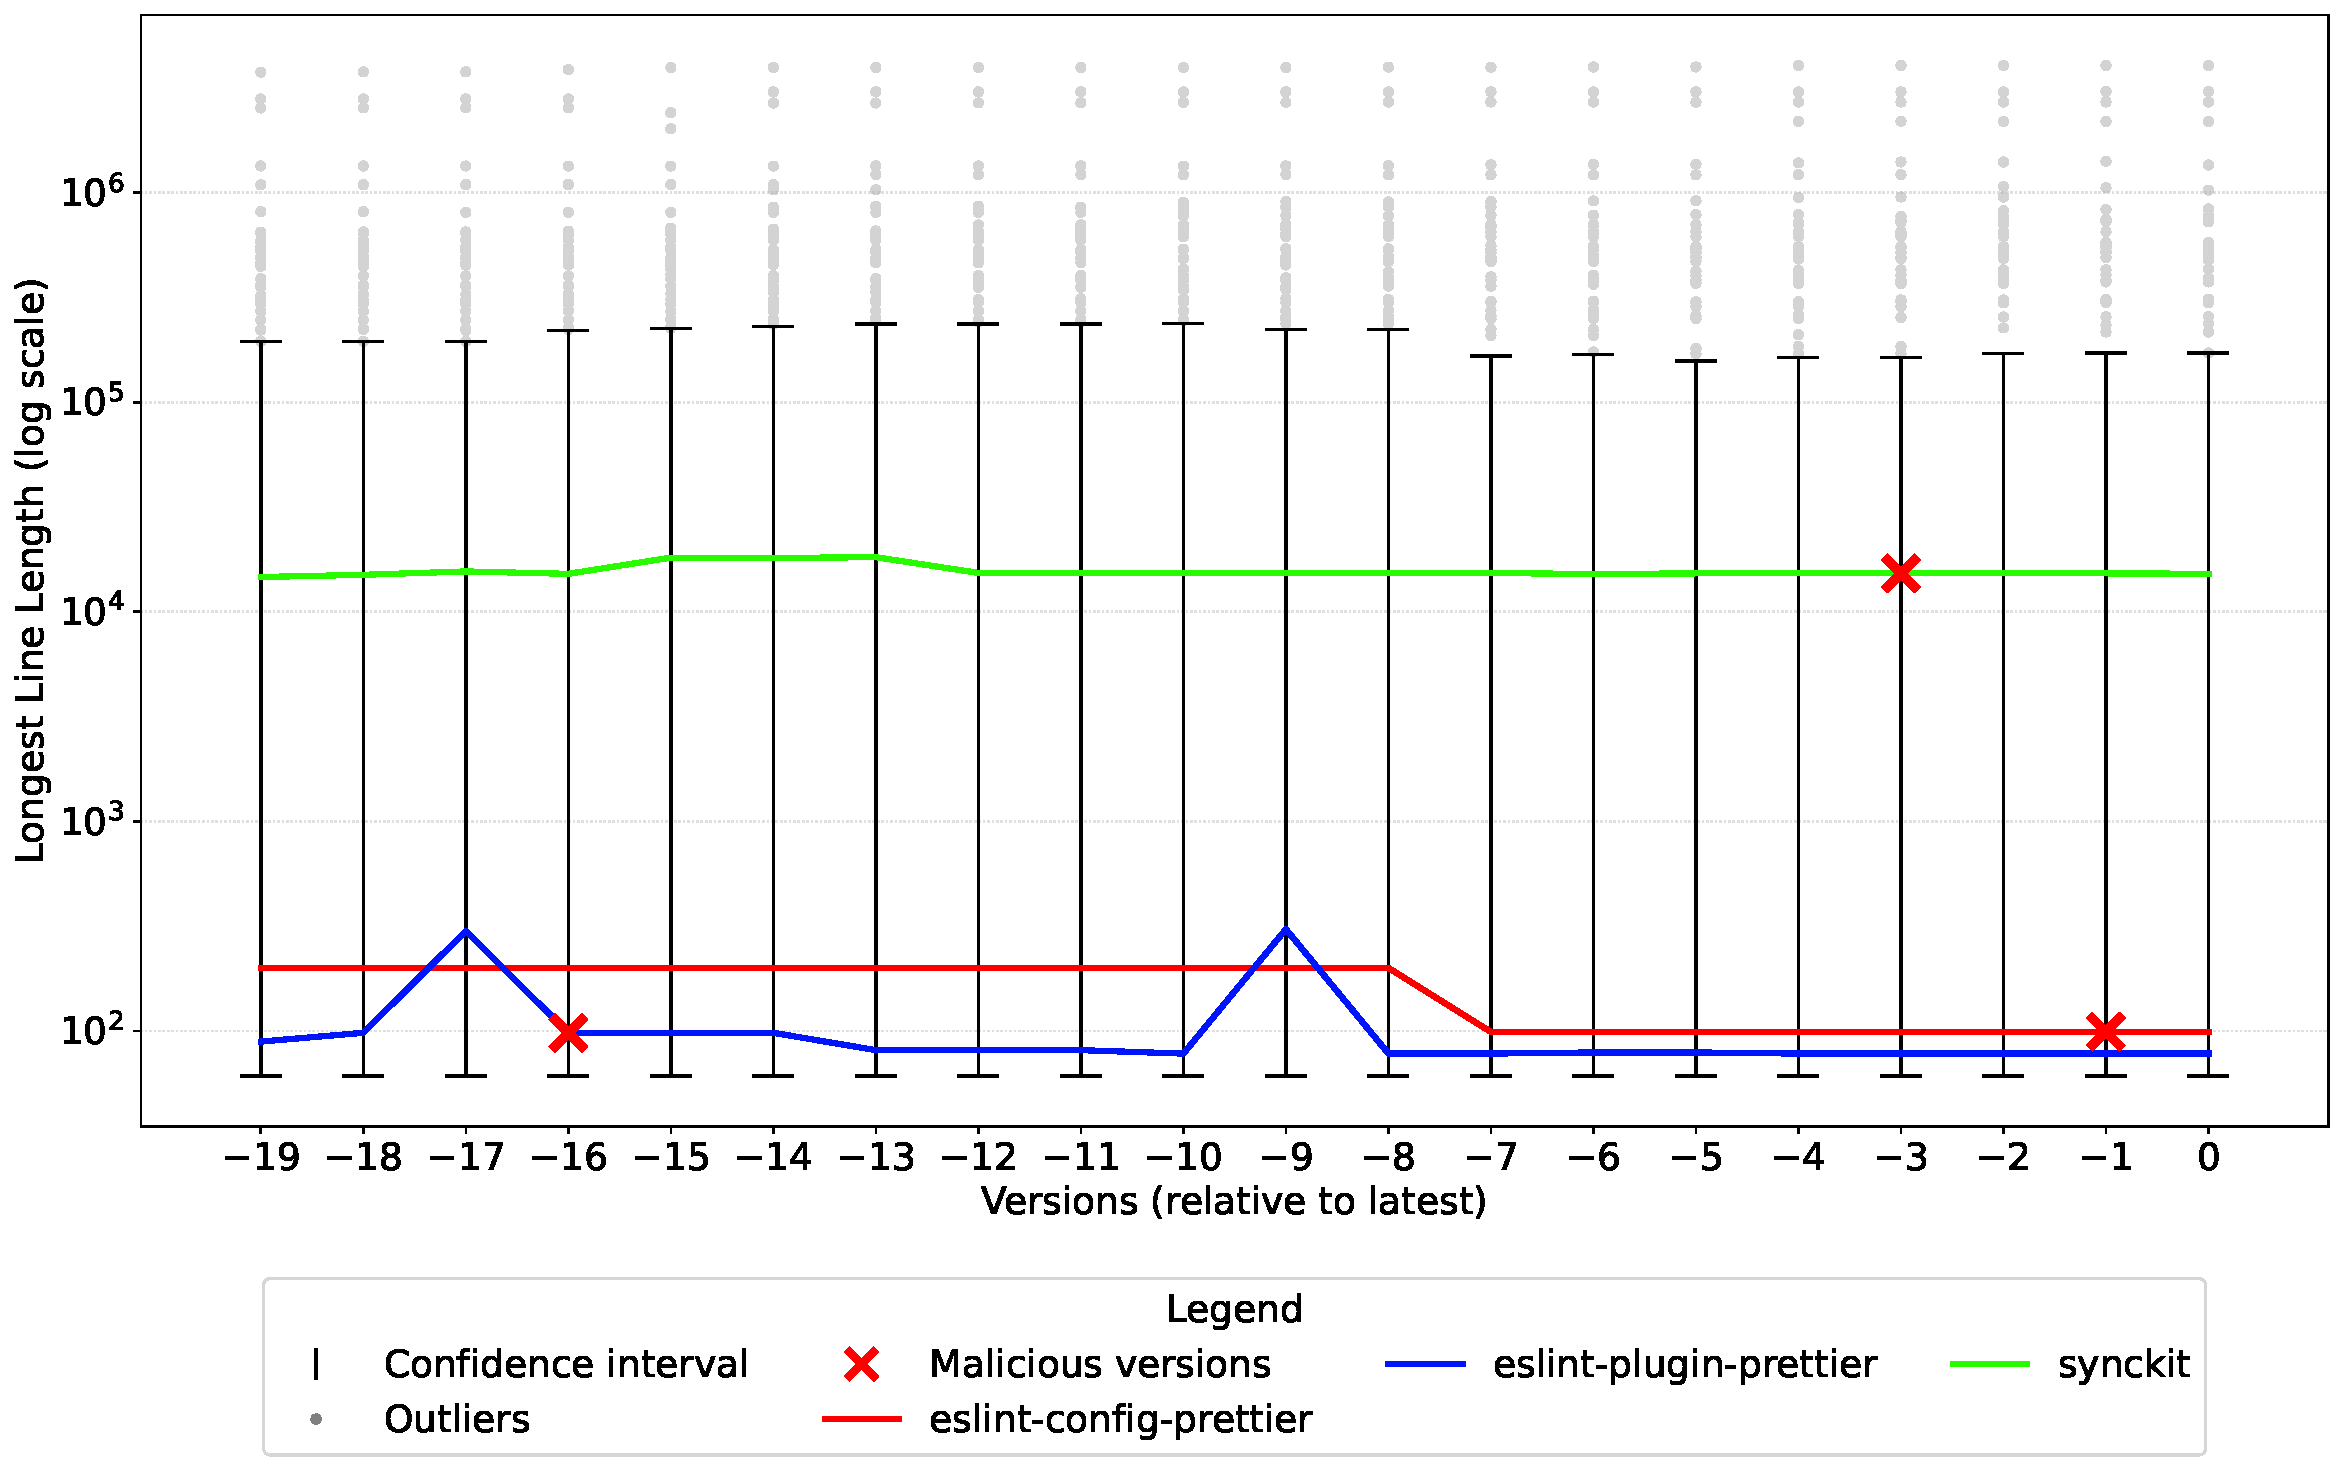
\includegraphics[width=\textwidth]{metrics/LongestLineLength/LLL_plot2single_AttackA.pdf}
    \caption{Comparison with Malware Dataset Longest Line Length Metric for Attack A}
    \label{fig:fig2LLLAttackA}
\end{figure}

In the first attack, the attacker inserted a malicious \ac{DLL} into the tarball (\cref{sec:attackA}),
without modifying or adding any plain text file.
Therefore, the longest line length remained unchanged compared to the legitimate versions,
as shown in \cref{fig:fig2LLLAttackA}.
Consequently, the metric is not indicative for detecting this specific attack.


\subsection*{Attack B: Crypto attack}
\label{sec:analysisLLLAttackB}

\begin{figure}[H]
    \centering
    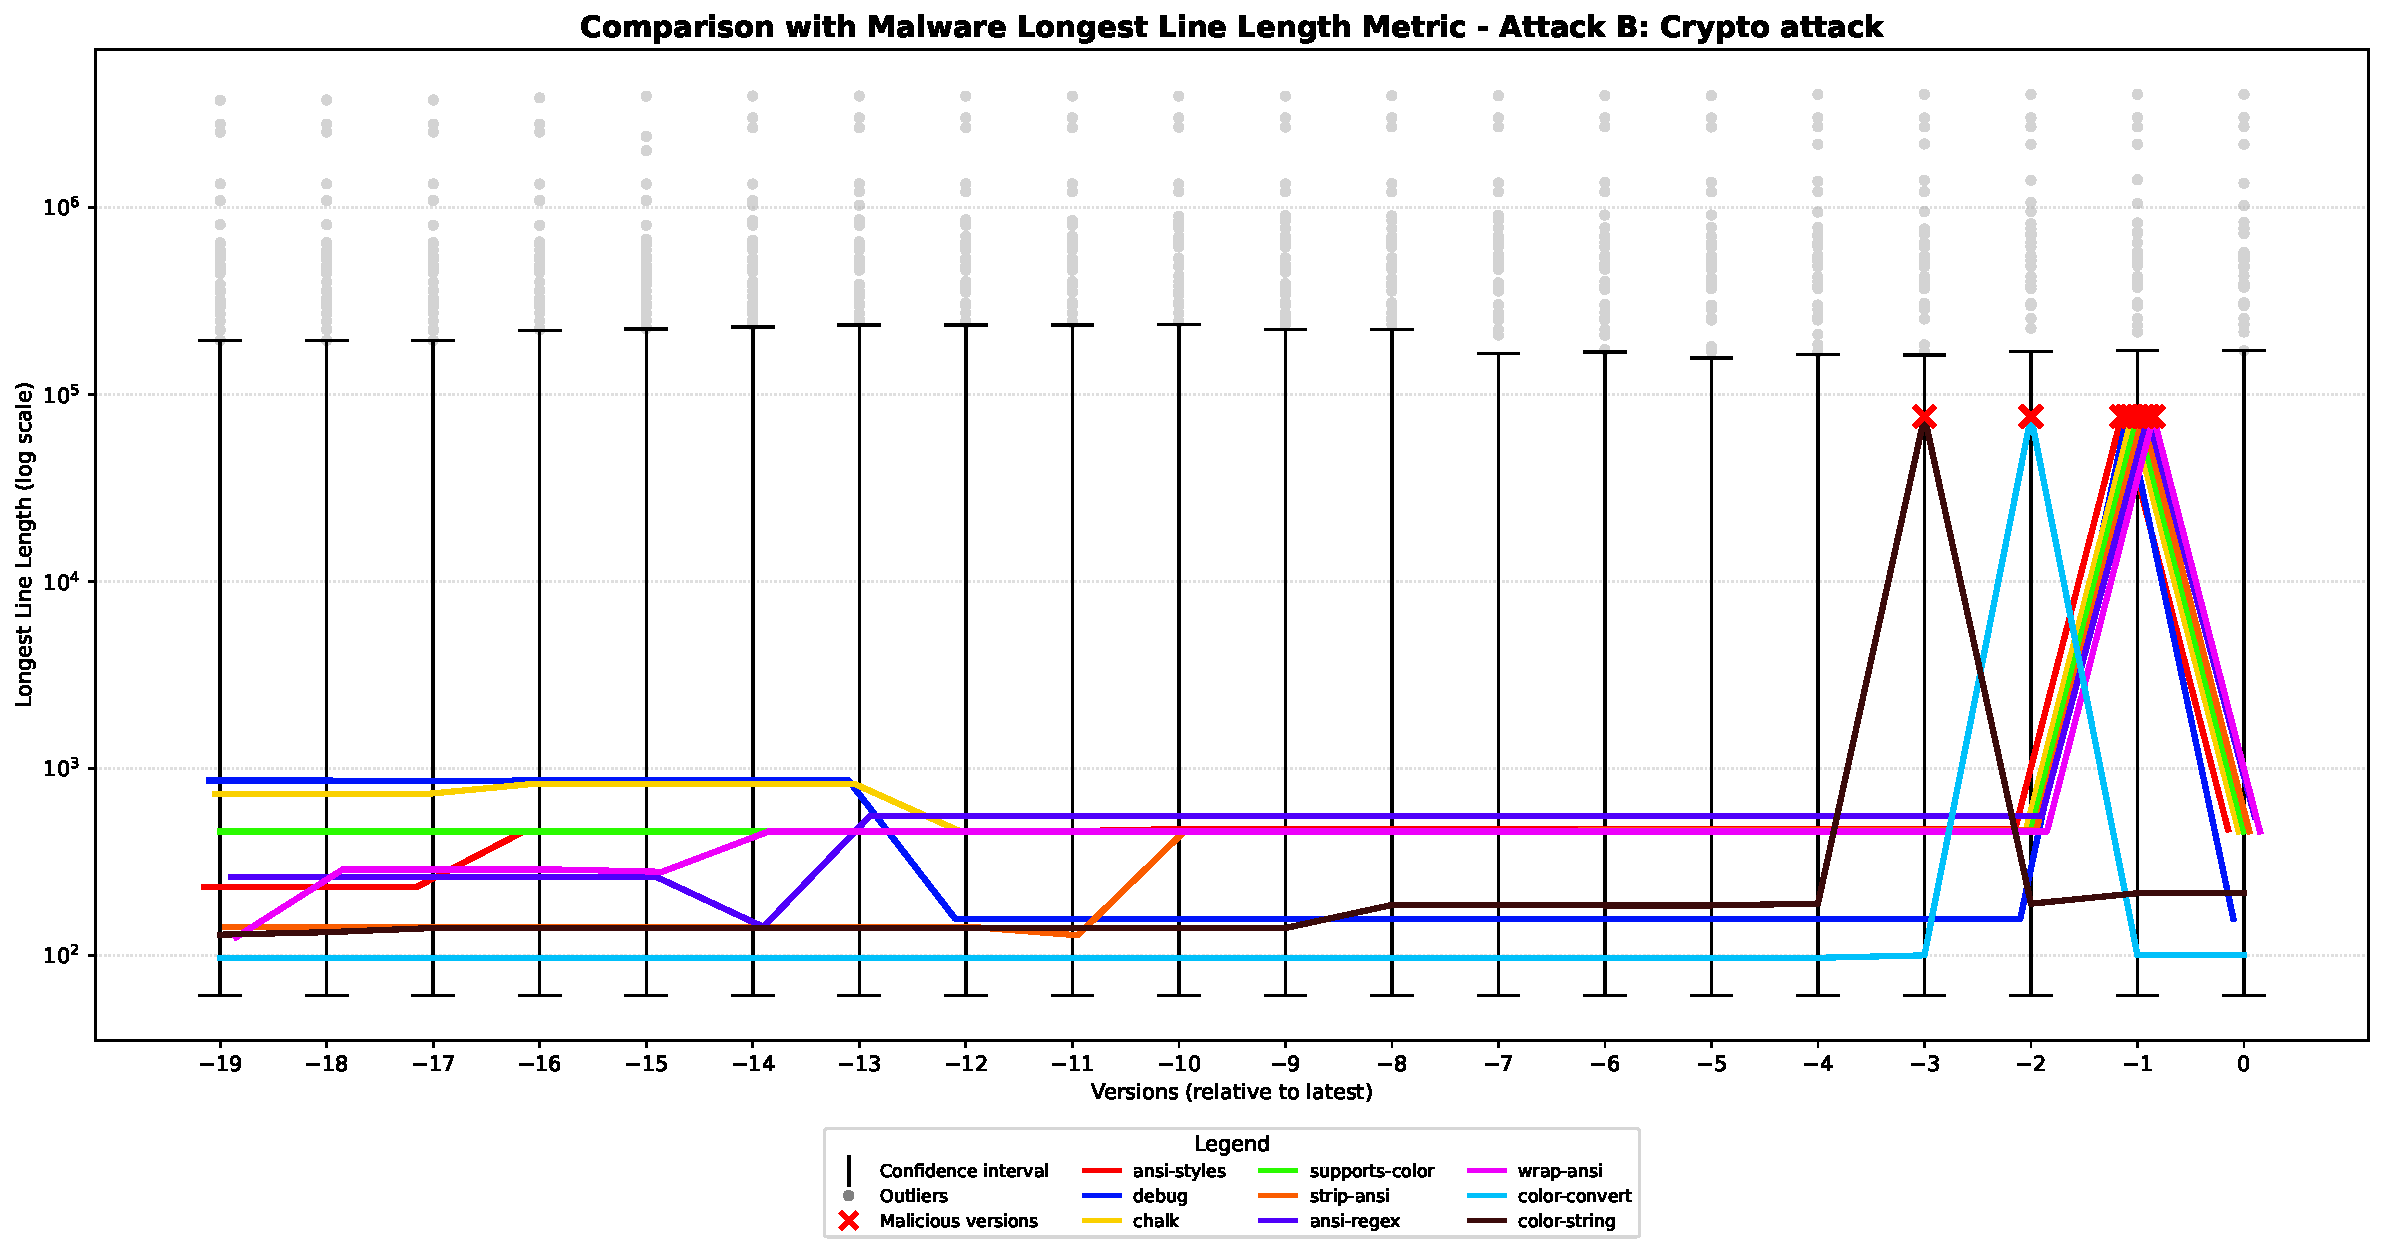
\includegraphics[width=\textwidth]{metrics/LongestLineLength/LLL_plot2single_AttackB.pdf}
    \caption{Comparison with Malware Dataset Longest Line Length Metric for Attack B}
    \label{fig:fig2LLLAttackB}
\end{figure}

Attack B (\cref{sec:attackB}) adds a single malicious line of 76,438 characters to the existing \texttt{index.js} file.
As shown in \cref{fig:fig2LLLAttackB}, the compromised versions exhibit a significant increase 
in the metric, but it is not sufficient to position them among the outlier values.
For this reason, the metric is not indicative for detecting this specific attack, as the 
malicious versions are indistinguishable from legitimate ones.

\subsection*{Attack C: Shai-Hulud 1.0}
\label{sec:analysisLLLAttackC}

\begin{figure}[H]
    \centering
    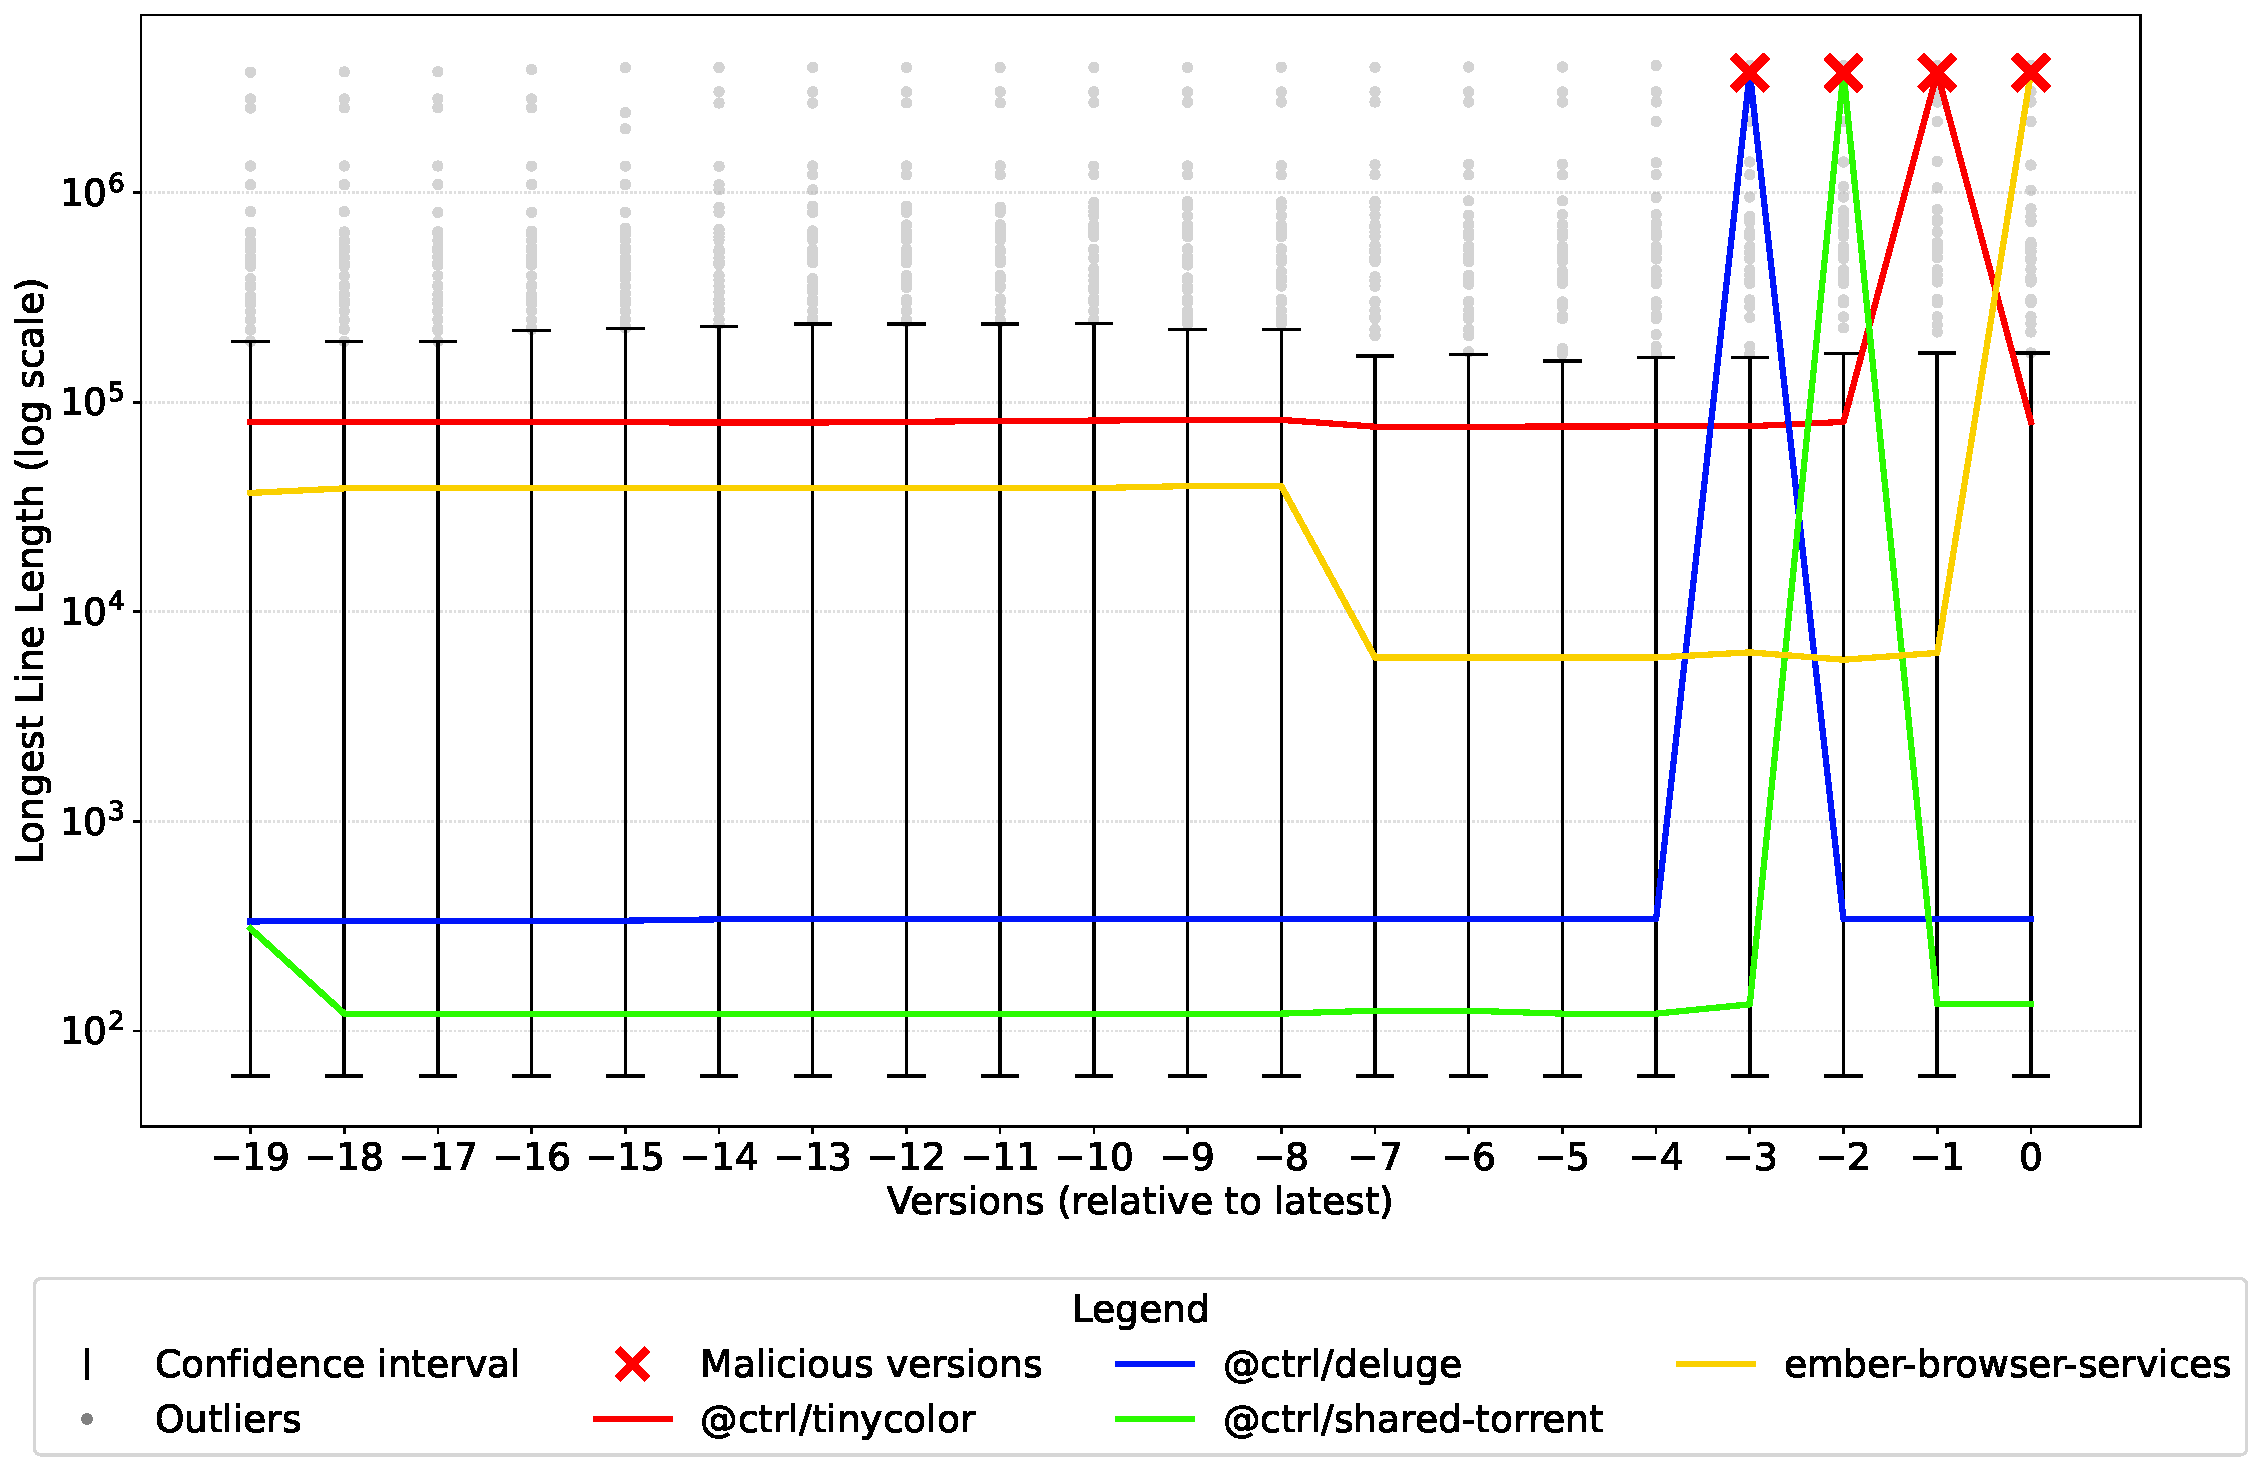
\includegraphics[width=\textwidth]{metrics/LongestLineLength/LLL_plot2single_AttackC.pdf}
    \caption{Comparison with Malware Dataset Longest Line Length Metric for Attack C}
    \label{fig:fig2LLLAttackC}
\end{figure}

In the third attack, the attacker introduced a malicious file named \texttt{bundle.js} 
(\cref{sec:attackC}) containing a single line of 3,734,355 characters.
As shown in \cref{fig:fig2LLLAttackC}, the malicious versions succeed in placing themselves 
among the outlier values, therefore the metric is effective for detecting this specific attack.

\subsection*{Attack D: Shai-Hulud 2.0}
\label{sec:analysisLLLAttackD}

\begin{figure}[H]
    \centering
    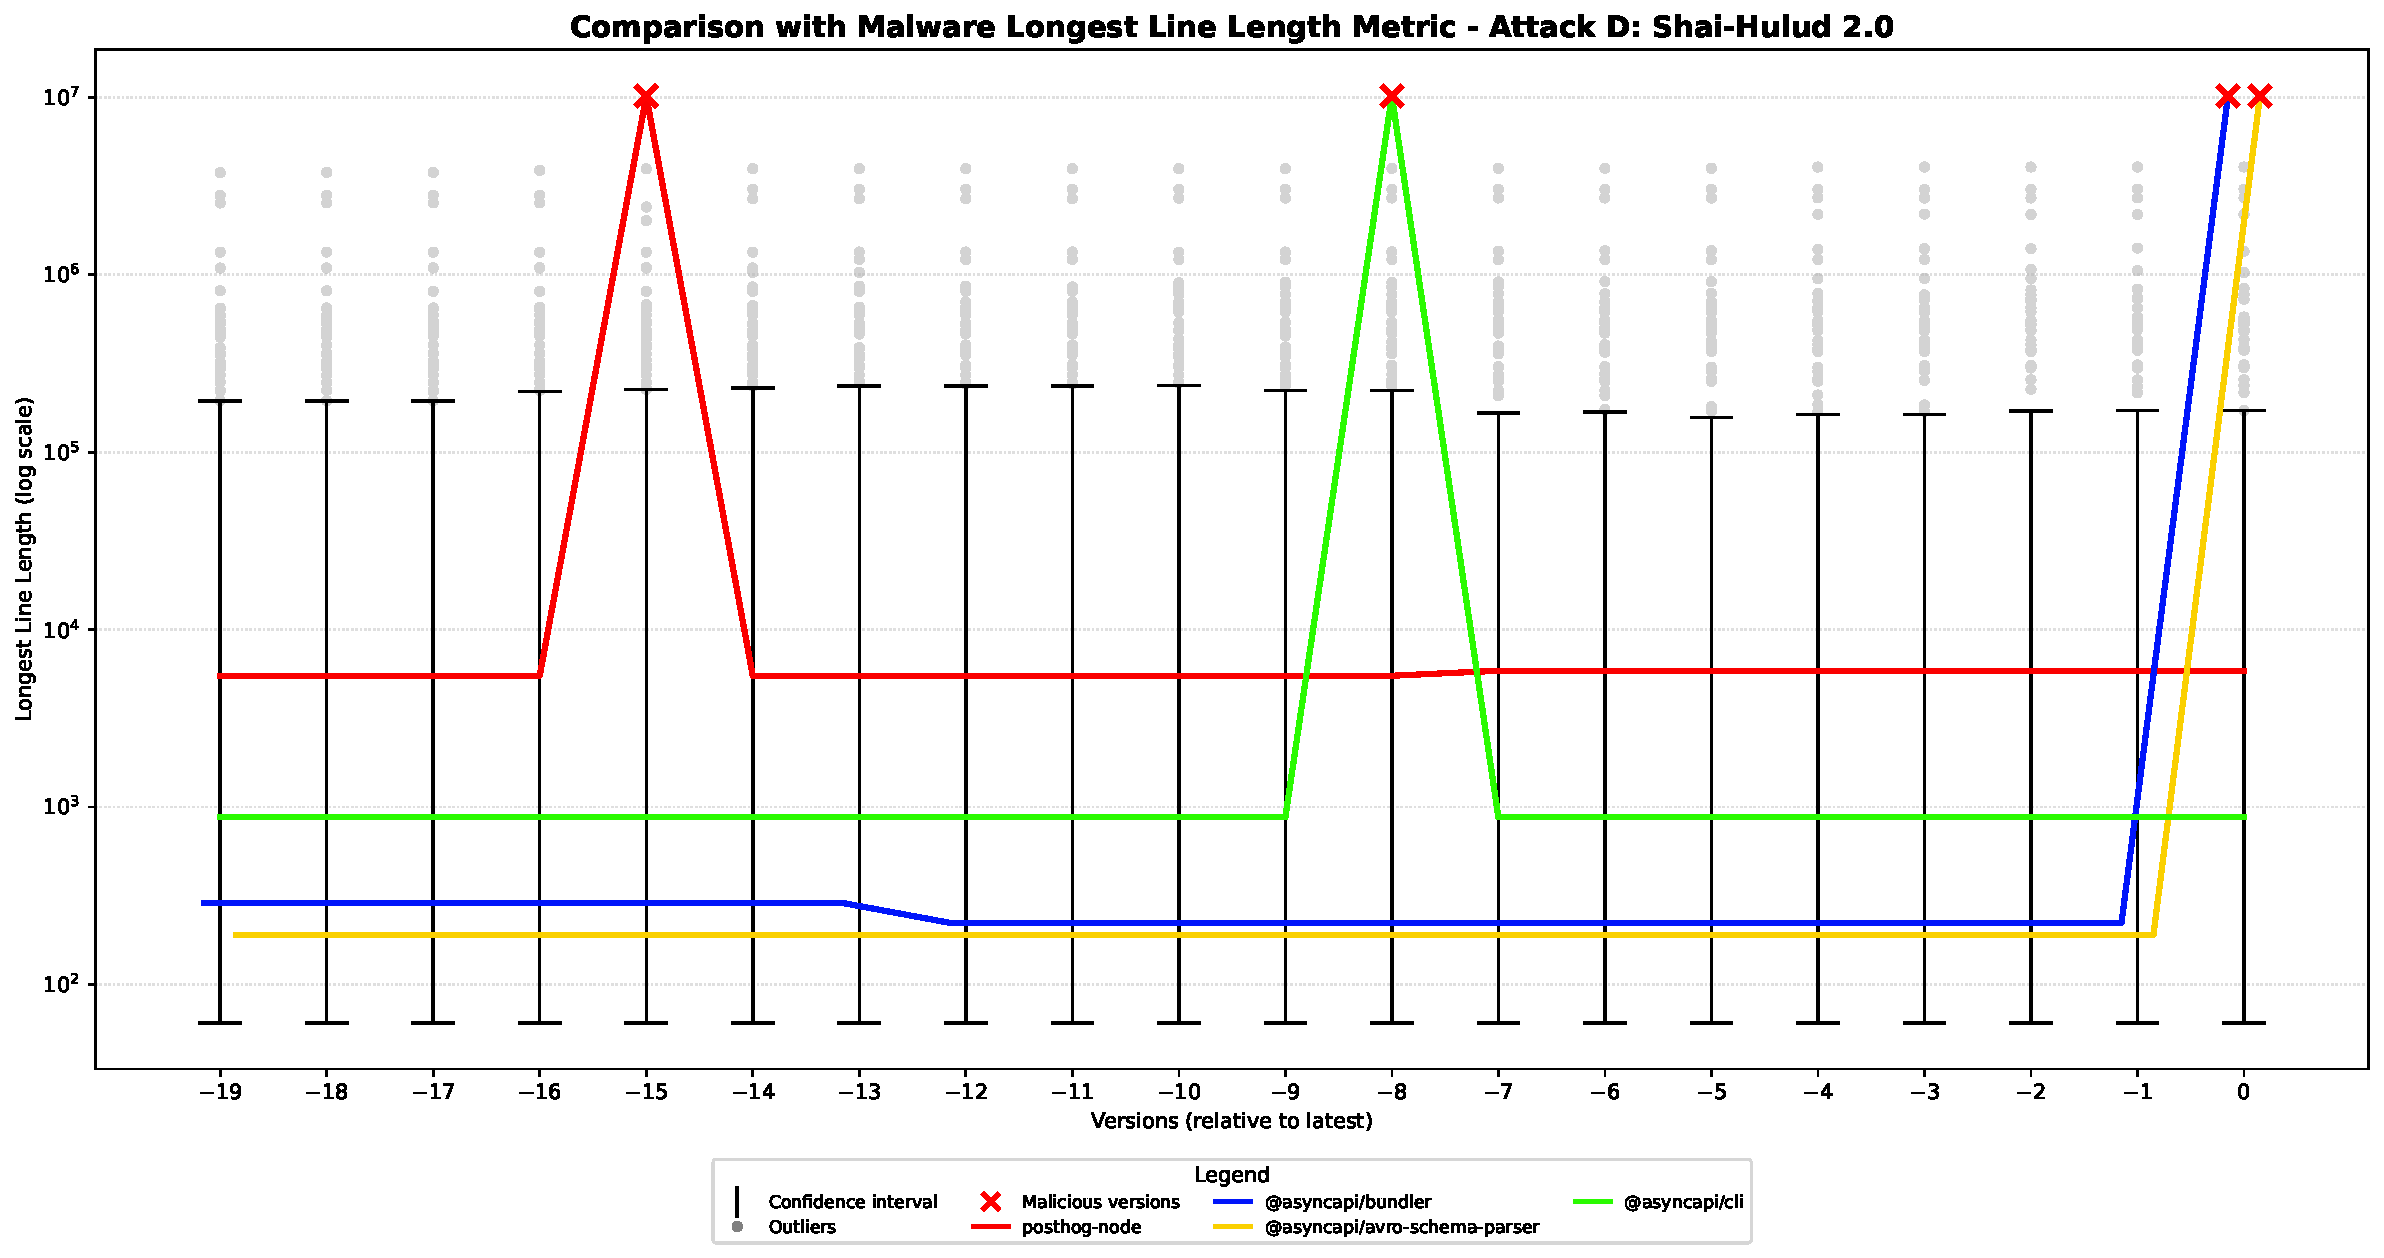
\includegraphics[width=\textwidth]{metrics/LongestLineLength/LLL_plot2single_AttackD.pdf}
    \caption{Comparison with Malware Dataset Longest Line Length Metric for Attack D}
    \label{fig:fig2LLLAttackD}
\end{figure}

Finally, in the fourth attack, the attacker introduces a malicious file named 
\texttt{setup\_bun.js} containing a single line of 10,157,373 characters (\cref{sec:attackD}).
As shown in \cref{fig:fig2LLLAttackD}, the malicious versions not only reach the outlier 
range but far exceed the maximum outlier values of the Goodware dataset.
Therefore, the metric is effective for detecting this attack.

\subsection*{Summary of Comparison with Malware Dataset}
\label{sec:analysisLLLSummaryComparisonMalware}

Despite this metric being influenced by the presence of build artifacts in the tarballs, 
it is possible to effectively detect the attack C (\texttt{Shai-Hulud}~1.0 \cref{sec:analysisLLLAttackC}) 
and the attack D (\texttt{Shai-Hulud}~2.0 \cref{sec:analysisLLLAttackD}), because in both cases the 
malicious versions introduce a malicious line whose length is sufficient to place them among 
the outlier values.

Instead, the metric is not indicative for detecting the attack A (Malicious Windows DLL \cref{sec:analysisLLLAttackA}),
because in this case the attacker did not modify or add any plain text file.
Furthermore, the metric is also not indicative for detecting the attack B (Crypto attack \cref{sec:analysisLLLAttackB}),
because in this case the malicious versions introduce a malicious line that is not 
long enough to place them among the outlier values, rendering them indistinguishable from legitimate versions.